\section{Estensione di Arcan per la detection dei nuovi smells}
    In questo capitolo viene effettuata una presentazione del \textit{tool} Arcan e delle modifiche necessarie per il riconoscimento dei tre nuovi \textit{architectural smells}. Oltre a una breve introduzione, vengono approfonditi diversi aspetti come la sua architettura e la struttura dati del grafo delle dipendenze. L'ultima sezione introduce le modifiche effettuate al \textit{tool} per rappresentare nel grafo le diverse strutture necessarie per il riconoscimento dei nuovi \textit{smell}.
        %La descrizione approfondita di Arcan viene effettuata nella sezione 3.1, che fornisce una breve introduzione al \textit{tool} e ne approfondisce differenti aspetti come le modalità di funzionamento, l'architettura con particolare enfasi sulla struttura dati del grafo delle dipendenze, gli AS che è in grado di ricercare all'interno del codice e le modifiche effettuate al grafo delle dipendenze per permettere la \textit{detection}. % degli \textit{smell} introdotti. 
    
    \subsection{Introduzione ad Arcan}
        Arcan (ARChitecture ANalizer) \cite{Arcan2017}\cite{Arcan2018} è uno strumento per l'analisi statica di sistemi software, sviluppato dal laboratorio Essere - Università degli Studi Milano Bicocca \cite{ESSeREwebsite}. Questo \textit{tool} è in grado di effettuare analisi statiche di programmi scritti in diversi linguaggi (Java, C, C++ e più recentemente Python \cite{stropeniPhdThesis}) al fine di calcolare differenti metriche ed effettuare la \textit{detection} di dieci tipologie di \textit{architectural smell}.  % (faccio la lista degli smell?). 
        %
        %Smell identificati da Arcan
        Non tenendo in considerazione i tre \textit{smell} introdotti in questo elaborato, Arcan è in grado di riconoscere i seguenti \textit{AS}:
        \begin{itemize}
            \item \textit{Cyclic Dependency} si riferisce a sottosistemi che sono coinvolti in catene di relazioni che non rispettano la natura aciclica della struttura delle dipendenze di un sottosistema, violando così il \textit{Acyclic Dependency Principle} \cite{martin2000design} \cite{Arcan2017}. %La presenza di questo smell obbliga le classi coinvolte ad essere riutilizzate e modificate insieme; potrebbe essere difficile inoltre anche la comprensione dei loro compiti, nel caso venissero analizzate singolarmente.
            
            \item \textit{Hub-Like Dependency} si verifica quando una \textit{abstraction} ha un alto numero di dipendenze in ingresso e in uscita, che non le permettono di mantenere accoppiamento basso e coesione alta \cite{Arcan2017}.
            %Questa abstraction quindi viola il principle of modularization e soprattutto non è in grado di garantire low coupling e high coesion \cite{SURYANARAYANA201521}.
            
            \item \textit{Unstable Dependency} riguarda sottosistemi (componenti) che dipendono da altri sottosistemi meno stabili di loro. Cambiamenti a sottosistemi che presentano dipendenze instabili possono causare modifiche a catena nel sistema \cite{Arcan2017}.
            
            \item \textit{God Component} si manifesta quando un componente è eccessivamente largo in termini di \textit{LOC (lines of code)} oppure numero di classi \cite{lippert2006refactoring}. 
            
            \item \textit{Insufficient Package Cohesion} descrive una situazione nella quale un entità architetturale presenta una coesione interna bassa.
            
            \item \textit{Feature Concentration} insorge quando un'entità architetturale implementa diverse funzionalità al suo interno \cite{deAndrade2014}.
            
            \item \textit{Scattered Funtionality} si presenta in un sistema dove diversi componenti sono responsabili della realizzazione delle stesse responsabilità di alto livello. \cite{Garcia2009}.
        \end{itemize}
        
    %
    %Architettura di Arcan
    \subsection{Architettura di Arcan}
        La struttura di Arcan è composta da quattro elementi principali \cite{Arcan2017}:
        %Arcan basa il suo funzionamento su quattro componenti principali \cite{Arcan2017}:
        \begin{enumerate}
            \item \textit{System Reconstructor} in grado di effettuare il \textit{parsing} del codice sorgente del progetto fornito come input e di estrarre da esso tutte le informazioni riguardanti le dipendenze tra i vari file, grazie all'utilizzo della libreria Spoon \cite{pawlak:hal-01169705}. Le informazioni estratte sono poi utilizzate per la generazione di una \textit{Abstract Syntax Tree (AST) map}. Questo componente non è in grado di recuperare eventuali dipendenze esterne al sistema e perciò Arcan è in grado di effettuare le analisi considerando solamente gli elementi passati come input.

            \item \textit{Graph Manager} è il componente responsabile della creazione del grafo delle dipendenze partendo dall'analisi della \textit{AST map} ricevuta dal \textit{System Reconstructor}. Dopo l'inizializzazione del grafo, inserisce in esso tutti i nodi e gli archi seguendo le dipendenze presenti nella mappa, contenenti le diverse informazioni riguardo i componenti del sistema sotto analisi. Questo componente utilizza la libreria Apache Tinkerpop \cite{ApahceTinkerpop} per svolgere le sue mansioni.
             
            \item \textit{Metrics Engine} si occupa della computazione delle metriche introdotte da R. Martin \cite{martin1994oometrics} necessarie per la detection degli \textit{architectural smells}. I risultati delle metriche calcolate vengono salvate poi all'interno dei componenti del grafo ai quali la metrica si riferisce.
            
            \item \textit{Architectural Smell Engine} contiene tutti gli algoritmi per la ricerca degli \textit{architectural smells} nel grafo e per il filtraggio dei falsi positivi. 
            Per ogni istanza trovata aggiunge un nuovo nodo di tipo \textit{smell} al grafo, che viene poi messo in relazione con i diversi nodi rappresentanti i componenti coinvolti in quella particolare istanza.
        \end{enumerate}
        
    \subsection{Grafo delle dipendenze}
        %Introduzione
        Il grafo delle dipendenze è l'elemento fondamentale su cui è basato tutto il funzionamento di Arcan. Si tratta di un \textit{graph database} che salva tutte le informazioni riguardanti il progetto analizzato attraverso gli elementi dei grafi (archi, nodi e anche le loro proprietà) e permette di svolgere \textit{graph computing} per effettuare il calcolo di metriche e il riconoscimento di \textit{AS}.
       % poichè svolge la funzione di database, immagazzinando all'interno dei vari elementi del grafo tutte le informazioni sul progetto, e permette l'identificazione degli smell e il calcolo delle diverse metriche, attraverso la \textit{graph computing}(?).
        %Il grafo delle dipendenze è un'elemento fondamentale per il funzionamento di Arcan poichè tutte le attività di identificazione di architectural smell e calcolo delle metriche vengono effettuate attraverso analisi del grafo generato dal componente \textit{Graph Manager}. 
    
    %Struttura del grafo
        Questo grafo si presenta come un grafo diretto, che mette in evidenza le dipendenze tra i vari componenti del progetto rappresentati dai nodi del grafo. Ogni nodo può rappresentare un elemento del linguaggio (package, classi, interfacce, funzioni e attributi) ed è in relazione con gli altri nodi tramite uno o più archi di diverse tipologie, che rappresentano al meglio la classificazione delle relazioni tra i componenti.  Nodi e archi possono presentare diverse proprietà utilizzate per il salvataggio di informazioni e metriche riguardanti un singolo componente.
            
    %Nodi e archi 
        Il grafo delle dipendenze dispone di numerose tipologie di nodi e archi, ma di seguito verranno presentate solamente gli elementi necessari per la comprensione del lavoro svolto. Le strutture riguardanti \textit{Attribute} e \textit{Function}, introdotte in questo elaborato e solamente accennate in questo elenco, hanno un approfondimento loro dedicato nelle sottosezioni 3.3.1 e 3.3.2.
        % Nodi
        Riguardo i nodi porremo la nostra attenzione solamente su quattro diverse tipologie:
        \begin{itemize}
            \item \textit{Unit}, classi concrete e astratte, interfacce ed enumerazioni. Queste tipologie di nodi sono descritti dagli attributi \textit{name}, \textit{filePath} e \textit{componentType}, che forniscono informazioni riguardanti rispettivamente il suo nome qualificato (compreso di \textit{namespace}), il percorso assoluto del file che contiene la \textit{unit} e la tipologia rappresentata. La proprietà \textit{componentType} può assumere i valori \textit{class}, \textit{abstract\_class}, \textit{interface} oppure \textit{enum}.  
            
            \item \textit{Smell}, tipologia di \textit{smell} identificata in una determinata \textit{unit}. Ogni diverso \textit{smell} definisce il suo particolare nodo, che contiene le diverse informazioni che lo caratterizzano. 
            
            \item \textit{Function}, singola funzione definita da una \textit{unit}.
            
            \item \textit{Attribute}, attributo contenuto in una \textit{unit}.
        \end{itemize}
        %Archi
        Tra le diverse tipologie di archi disponibili, quelle importanti per lo sviluppo della detection e la comprensione degli algoritmi sono:
        \begin{enumerate}
            \item \textit{dependsOn} collega due nodi di tipo \textit{unit}, e indica che il nodo con questo arco in uscita ha una dipendenza verso l'altra \textit{unit}. Un esempio di dependsOn potrebbe essere una classe che al suo interno richiama i metodi di un'altra classe.
            
            \item \textit{isChildOf} è indice di una relazione di tipo gerarchico tra due diverse \textit{unit}, con il supertipo che presenta questo arco in entrata. %In particolare la unit che ha questo arco in entrata è il supertipo mentre l'altra è, di conseguenza, un sottotipo.
            
            \item \textit{isImplementationOf} raffigura l'implementazione da parte di una \textit{unit} di un'interfaccia. Nel dettaglio la \textit{unit} che ha l'arco isImplementationOf in uscita implementa l'interfaccia rappresentata dall'altra \textit{unit}.
            
            \item \textit{containedIn} definisce una relazione tra una \textit{unit} e un attributo che essa definisce.
            
            \item \textit{implementedBy} che rappresenta l' implementazione di una funzione da parte di una \textit{unit} specifica. 
            
            \item \textit{affects} indica che l'istanza di uno \textit{smell}, che possiede questo arco in uscita, è stata trovata in una determinata \textit{unit}. %nella unit che presenta l'arco in ingresso.
            
            \item \textit{archi di tipologie particolari}, definite dagli \textit{smell} per rappresentare diverse situazioni particolari. Vengono utilizzati in combinazione con l'arco \textit{affects}.
            
            %Ogni nodo \textit{smell} può presentare, oltre all'arco \textit{affects}, anche altri \textit{archi di tipologie particolari} e significative per quella tipologia di \textit{smell}.
        \end{enumerate}
    
    \subsection{Modifiche effettuate al grafo}
        Al fine di implementare la \textit{detection} degli \textit{smell} introdotti, è stata necessaria la modifica degli algoritmi di \textit{parsing} esistenti e l'aggiunta di nuove strutture al grafo delle dipendenze. Nello specifico sono state effettuate modifiche al \textit{parser} Java per il recupero di informazioni riguardanti funzioni e attributi e introdotte nel grafo le strutture necessarie per la loro rappresentazione.
        
        \subsubsection{Parsing e rappresentazione di funzioni}
        %Introduzione
            Il ruolo delle funzioni nelle strategie di identificazione è fondamentale per tutti e tre gli algoritmi presentati.
            %La funzioni svolgono un ruolo fondamentale in tutti e tre le strategie di identificazione per gli smell presentati, quindi l'introduzione di queste modifiche è stata necessaria per l'implementazione di tutti e tre gli algoritmi. 
            
            Arcan disponeva già della struttura necessaria per il \textit{parsing} delle funzioni, perciò è stato necessario solamente effettuare l'implementazione degli algoritmi per il recupero delle informazioni utilizzando le API fornite dalla libreria Spoon \cite{pawlak:hal-01169705}. 

            %Dettaglio aggunte
            Le modifiche al grafo per la rappresentazione delle funzioni hanno comportato l'introduzione di due nuovi tipi di componenti, un nodo \textit{function} e un arco implementedBy. Il nodo \textit{function} rappresenta la singola funzione definita da una classe o interfaccia, dove il valore della proprietà \textit{name} del nodo corrisponde al nome della funzione rappresentata dallo stesso. Per rappresentare la definizione di una funzione da parte di una \textit{unit} è stato introdotto un arco di tipo \textit{implementedBy}, in uscita dalla funzione verso la \textit{unit} che la contiene.
            %Un'arco di tipo \textit{implementedBy} è stato introdotto al fine di identificare la unit che definisce una determinata funzione; questo arco è in uscita dal nodo della funzione verso appunto la unit che lo contiene. 
            Un esempio di questa struttura si può identificare nella figura 1 dove la funzione è rappresentata dal nodo verde e la \textit{unit} che la implementa da quello di colore beige. 
            
            Durante la modifica del \textit{parsing} è stato necessario effettuare due scelte principali: la rappresentazione delle funzioni non per \textit{signature} ma per nome e la tecnica di recupero dei metodi definiti.
            
            %Scelta funzioni definite solo dal nome
            La scelta di rappresentare le funzioni attraverso il nome è stata effettuata al fine di favorire la detection dello \textit{smell} \textit{Subclasses Do Not Redefine Method} (sezione 4.1), dove viene controllato che il sottotipo ridefinisca almeno un metodo del suo supertipo. In particolare si desiderava l'inclusione anche di tutti i casi di \textit{overloading}, dove un figlio non ridefinisce il comportamento di un metodo che il padre implementa ma aggiunge un nuovo comportamento per un metodo già esistente, rappresentato da supertipo e sottotipo che condividono un metodo con lo stesso nome ma con \textit{signature} differente.
            
            %Scelta parsing solo funzioni implementate
            La libreria Spoon \cite{pawlak:hal-01169705} utilizzata per il \textit{parsing} presenta inoltre due differenti tipologie di recupero delle funzioni da una determinata classe e/o interfaccia del sistema:
            \begin{enumerate}
                \item Recupero dei metodi definiti direttamente dal componente.
                
                \item Recupero delle funzioni che possono essere chiamati su un istanza di quel componente, inclusi quindi anche tutti i metodi derivati dalle superclassi.
            \end{enumerate}
            È stato preferito il primo approccio poiché il secondo presentava diverse criticità. Nel linguaggio Java tutte le classi derivano dalla classe \textit{Object} e quindi le funzioni di quest'ultima sarebbero risultate implementate da tutte le \textit{unit}, con conseguenza che nessuna di esse sarebbe risultata come \textit{smell} \textit{Subclasses Do Not Redefine Methods} (sezione 4.1). Inoltre questa soluzione avrebbe portato a un eccessivo appesantimento del grafo e di Arcan in generale, poiché oltre ai metodi di \textit{Object} aggiunti a tutte le classi ogni funzione sarebbe stata replicata per tutte le \textit{unit} che la ereditano.
        
        
        \subsubsection{Parsing e rappresentazione di attributi}
            Arcan non disponeva di nessuna struttura o algoritmo dedicata al \textit{parsing} degli attributi, perciò tutte le classi e algoritmi sono stati implementati da zero, considerando comunque la struttura degli altri elementi simili per garantire continuità nel codice.
            La presenza nel grafo di informazioni riguardanti gli attributi definiti dalle \textit{unit} è stata necessaria per il riconoscimento dello \textit{smell} \textit{Unnecessary Abstraction}.
            Questa esigenza ha portato all'introduzione nel grafo di due nuovi elementi: un nodo di tipo \textit{attribute} e un arco \textit{containedIn}. Il nodo \textit{attribute} rappresenta un attributo definito da una particolare classe, collegato con un arco in ingresso verso la \textit{unit} che lo definisce. Un esempio della struttura è presentato dalla figura 1, dove il nodo di colore beige rappresenta la \textit{unit} mentre quello rosa l'attributo.
            
            Un attributo può essere inoltre identificato univocamente all'interno del grafo grazie alla proprietà \textit{name}, formata dalla concatenazione del nome della classe che lo definisce e quello dell'attributo stesso. Questi nodi presentano inoltre tre proprietà aggiuntive rispetto agli altri:
            \begin{itemize}
                \item \textit{Attribute type}, tipo dell'attributo rappresentato dal nodo (può essere sia un tipo primitivo che il nome qualificato di una classe)
                \item \textit{Constant attribute}, \textit{flag} che indica se è un valore costante o meno
                \item \textit{Default value}, \textit{flag} che specifica la presenza o meno di un valore assegnato
            \end{itemize}
            
        \subsubsection{Modifiche alla classe Unit}
            Un ulteriore elemento che ha subito modifiche è la classe Unit, rappresentante di un nodo \textit{unit} del grafo, che ha visto l'aggiunta di diverse procedure per il recupero di metodi e attributi definiti. È stato introdotta la funzione \textit{getAllMethods}, che produce in output tutti i metodi concreti o astratti definiti nella gerarchia di una \textit{unit}, al fine di considerare per lo \textit{smell} \textit{Subclasses Do Not Redefine Methods} anche tutte le funzioni ereditate. 
            %Vengono recuperate inoltre anche le procedure definite dalle interfacce implementate da classi astratte, poiché esse non sono obbligate a definire tutti i metodi dell'interfaccia ma vengono comunque considerati come definiti dai supertipi.
            In Java inoltre le classi astratte che implementano un'interfaccia non sono obbligate alla definizione di tutti i suoi metodi e la loro implementazione viene lasciata alle classi concrete che estendono quella astratta. È stato deciso quindi di considerare queste funzioni come definite comunque dalle classi astratte, come fossero metodi \textit{abstract}, e vengono quindi recuperate dalla procedura \textit{getAllMethods}.
            %\paragraph{Altre modifiche} 
            %Oltre all'introduzione di nuove strutture nel grafo e alle modifiche al \textit{parser}, anche altri elementi di Arcan hanno ricevuto modifiche minori:
            %\begin{itemize}
                % Aggiunta delle inner classes, postprocessor per il problema delle interfacce\\
            \defaultvspace
            \defaultvspace
            \defaultvspace
            \begin{figure}[h]
                \centering
                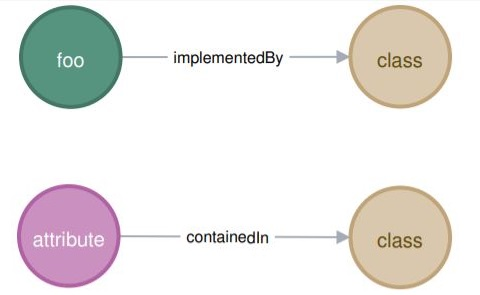
\includegraphics[scale=0.8]{Tesi/Sezione3-RiconoscimentoSmell/immagini/Cattura3.jpg}
                \caption{Esempio di strutture per attributi e funzioni}
            \end{figure}    
